\begin{figure}[htpb]
    \centering
    \begin{subfigure}[t]{0.45\textwidth}
    \centering
    \label{fig:gru}
    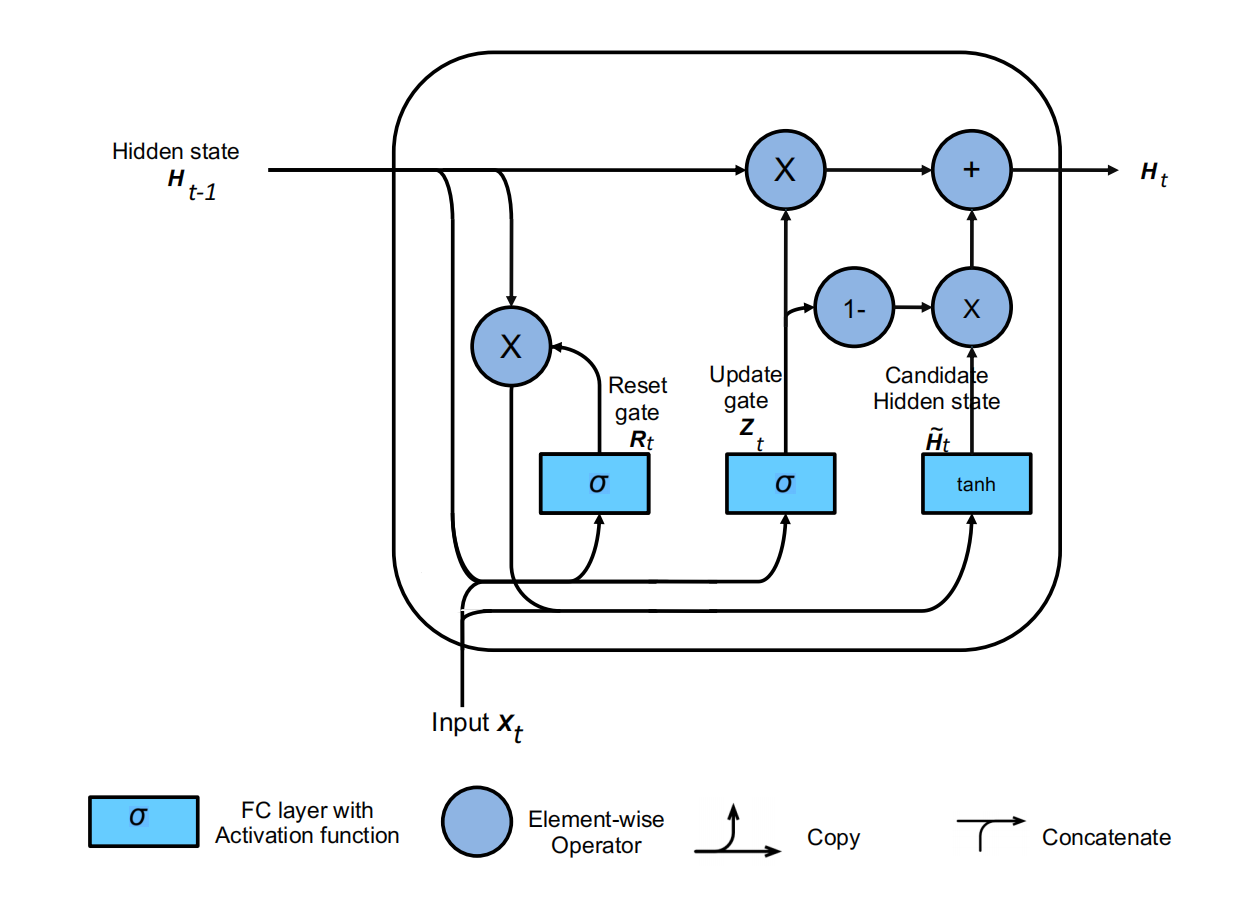
\includegraphics[width=\textwidth]{figs/gru.png}
    \caption{GRU (Gated recurrent units)}
    {\footnotesize
    $\mathbf{H}_t
    = \mathbf{Z}_t\odot\mathbf{H}_{t-1}
    + (1-\mathbf{Z}_t)\odot\Tilde{\mathbf{H}}_t$
    }
    \end{subfigure}
    \begin{subfigure}[t]{0.45\textwidth}
    \centering
    \label{fig:lstm}
    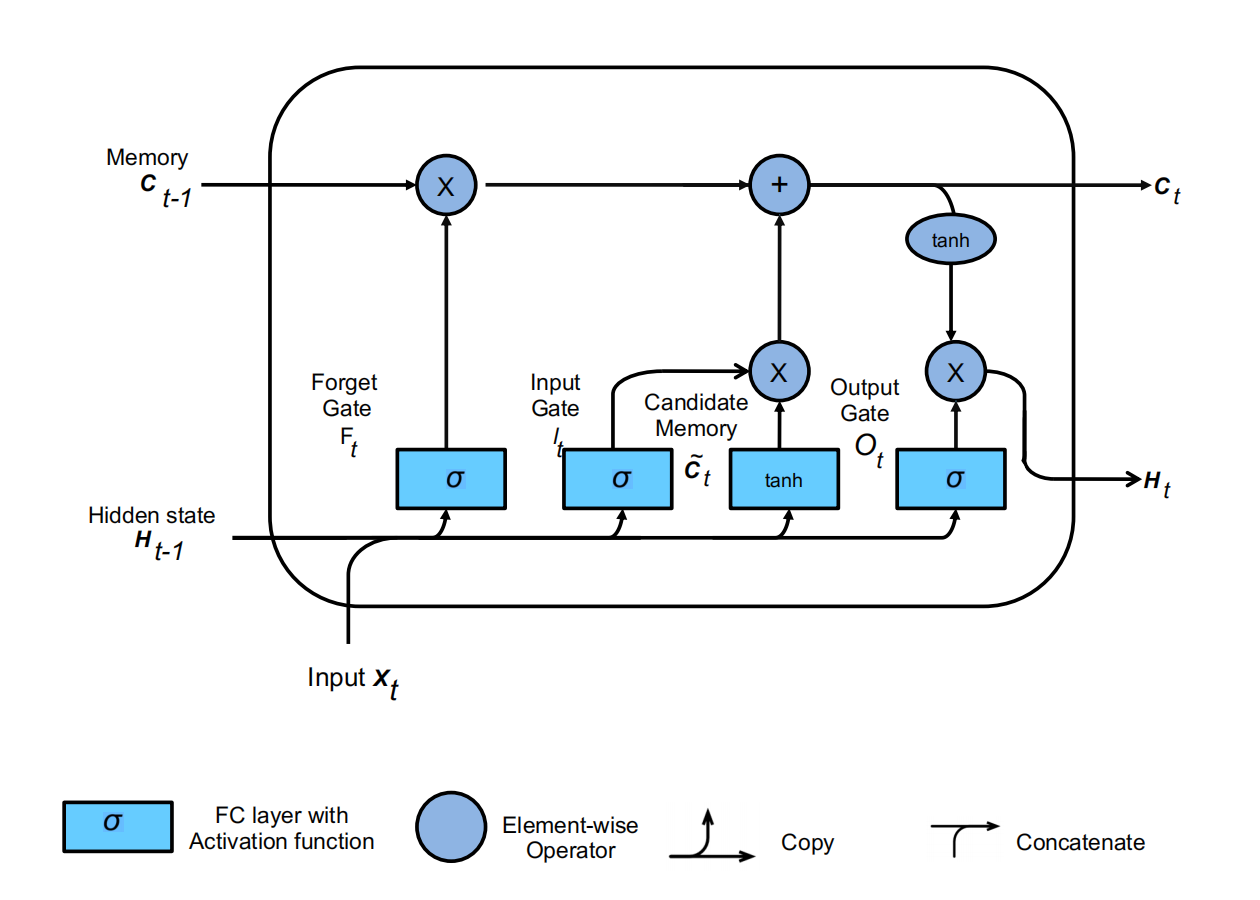
\includegraphics[width=\textwidth]{figs/lstm.png}
    \caption{LSTM (Long short term memory)}
    {\footnotesize
    $\mathbf{C}_t=\mathbf{F}_t\odot\mathbf{C}_{t-1}+\mathbf{I}_t\odot\Tilde{\mathbf{C}}_t$\\
    $\mathbf{H}_t=\mathbf{O}_t\odot\mathrm{tanh}(\mathbf{C}_t)$
    }
    \end{subfigure}
    \caption{Gating and long term momory}
    {\footnotesize
    Since gradient vanishing, the vanilla RNNs fail to remember inputs from long in the past.
    The problem is solved by specify the update of hidden state.
    }
    \label{fig:grulstm}
\end{figure}



